\apendice{Documentación de usuario}

\section{Introducción}
Este documento detalla cómo un usuario, puede utilizar la aplicación una vez desplegada en un servidor.
\section{Requisitos de usuarios}
Los requisitos para poder utilizar la aplicación son:
\begin{itemize}
	\tightlist
	\item Tener la aplicación desplegada en algún servidor.
	\item Disponer de conexión al servidor y tener instalado un navegador web con el que poder acceder a la aplicación. Se recomienda:
	\begin{itemize}
		\tightlist
		\item Google Chrome Versión 75.0.3770.100 o superior
		\item Firefox Quantum Versión 67.0.4 o superior
		\item IE11 Versión 11.829.17134.0 o superior
		\item Opera Versión:62.0.3331.18 o superior
	\end{itemize}
\end{itemize}
\section{Instalación}
Al ser una aplicación web no requiere instalación. Solo es necesario desplegar la aplicación en un servidor.
\section{Manual del usuario}
La aplicación permite añadir proyectos de GitLab y evaluarlos mediante métricas de evolución.\\
\subsection{Conceptos}
Para utilizar la aplicación es importante entender los siguientes conceptos:\\
\textbf{\textit{Medición}}\\
El proceso de medición es un proceso en el que se asignan números o símbolos a atributos de entidades del mundo real, de tal forma que los caracteriza a través de reglas.\\
\textbf{\textit{Métrica}}\\
Medida cuantitativa del grado en que un sistema, componente o proceso posee un atributo dado (IEEE, 1993).\\
\textbf{\textit{Indicador}}\\
Métrica o combinación de métricas que proporcionan una visión profunda del proceso, del proyecto o del producto.\\
\textbf{\textit{Métrica de evolución}}\\
Es una métrica que mide un atributo del proceso de desarrollo de un producto software.\\
\textbf{\textit{Evaluación}}\\
Es uno de los objetivos del proceso de medición. Consiste en determinar el estado de un proyecto en relación con otros proyectos de la misma naturaleza.\\
\textbf{\textit{Proyecto (software)}}\\
Proyecto en el cual se desarrolla un producto software.\\
\textbf{\textit{Repositorio de código}}\\
Lugar dónde se almacena el código de un proyecto software. A menudo cuentan con un sistema de control de versiones.\\
\textbf{\textit{Sistema de control de veriones (VCS - Version Control System)}}\\
Sistema que registra los cambios que se producen sobre los ficheros de un proyecto software almacenados en un repositorio de código.\\
\textbf{\textit{Sistema de seguimiento de incidencias (Issue tracking system)}}\\
Sistema que gestiona las diferentes tareas o incidentes que se definen en un proyecto software y que pueden ser asignadas a colaboradores del proyecto.

\subsubsection{Las métricas que se gestionan en la aplicación}
Las métricas que se calculan de los proyectos son un conjunto de métricas que proceden de la Master Tesis titulada \textit{sPACE: Software Project Assessment in the Course of Evolution} \cite{ratzinger_space:_2007}.\\\\
\textbf{\underline{I1 - Número total de issues}}
\begin{itemize}
	\tightlist
	\item \textbf{Categoría}: Proceso de Orientación
	\item \textbf{Descripción}: Número total de issues creadas en el repositorio
	\item \textbf{Propósito}: ¿Cuántas issues se han definido en el repositorio?
	\item \textbf{Fórmula}: NTI. NTI = número total de issues
	\item \textbf{Fuente de medición}: Repositorio de un gestor de repositorios
	\item \textbf{Interpretación}: NTI >= 0. Valores bajos indican que no se utiliza un Sistema de seguimiento de incidencias, podría ser porque el proyecto acaba de comenzar
	\item \textbf{Tipo de escala}: Absoluta
	\item \textbf{Tipo de medida}: NTI = Contador
\end{itemize}
\textbf{\underline{I2 - Commits por issue}}
\begin{itemize}
	\tightlist
	\item \textbf{Categoría}: Proceso de Orientación
	\item \textbf{Descripción}: Número de commits por issue
	\item \textbf{Propósito}: ¿Cuántos commits realizados por cada issue?
	\item \textbf{Fórmula}: CI = NTC/NTI. NTI = Numero total de issues, NTC = Número total de commits
	\item \textbf{Fuente de medición}: Repositorio de un gestor de repositorios
	\item \textbf{Interpretación}: CI >= 0, Si se acerca a 1 se definen bien las issues, si alto: no se definen bien las issues, si bajo: desarrollo del proyecto lento
	\item \textbf{Tipo de escala}: Ratio 
	\item \textbf{Tipo de medida}: NTI, NTC = Contador
\end{itemize}
\textbf{\underline{I3 - Porcentaje de issues cerradas}}
\begin{itemize}
	\tightlist
	\item \textbf{Categoría}: Proceso de Orientación
	\item \textbf{Descripción}: Porcentaje de issues cerradas
	\item \textbf{Propósito}: ¿Qué porcentaje de issues definidas en el repositorio se han cerrado?
	\item \textbf{Fórmula}: PIC = NTIC*100/NTI. NTIC = Número total de issues cerradas, NTI = Numero total de issues
	\item \textbf{Fuente de medición}: Repositorio de un gestor de repositorios
	\item \textbf{Interpretación}: 0 <= PIC <= 100. Cuanto más alto mejor
	\item \textbf{Tipo de escala}: Ratio
	\item \textbf{Tipo de medida}: NTI, NTIC = Contador
\end{itemize}
\textbf{\underline{TI1 - Media de días en cerrar una issue}}
\begin{itemize}
	\tightlist
	\item \textbf{Categoría}: Constantes de tiempo
	\item \textbf{Descripción}:  Media de días en cerrar una issue
	\item \textbf{Propósito}: ¿Cuánto se suele tardar en cerrar una issue? 
	\item \textbf{Fórmula}: MDCI = SUM(DCI) / NTIC . NTIC = Número total de issues cerradas, DCI = Días en cerrar la issue
	\item \textbf{Fuente de medición}: Repositorio de un gestor de repositorios
	\item \textbf{Interpretación}: MDCI >= 0. Cuanto más pequeño mejor.
	\item \textbf{Tipo de escala}: Ratio
	\item \textbf{Tipo de medida}: NTI, NTIC = Contador
\end{itemize}
\textbf{\underline{TC1 - Media de días entre commits}}
\begin{itemize}
	\tightlist
	\item \textbf{Categoría}: Constantes de tiempo
	\item \textbf{Descripción}: Media de días que pasan entre dos commits consecutivos
	\item \textbf{Propósito}: ¿Cúanto tiempo suele pasar desde un commit hasta el siguiente?
	\item \textbf{Fórmula}: MDEC = [Sumatorio de (TCi-TCj) desde i=1, j=0 hasta i=NTC] / NTC. NTC = Número total de commits, TC = Tiempo de Commit 
	\item \textbf{Fuente de medición}: Repositorio de un gestor de repositorios
	\item \textbf{Interpretación}: MDEC >= 0. Cuanto más pequeño mejor.
	\item \textbf{Tipo de escala}: Ratio
	\item \textbf{Tipo de medida}: NTC = Contador; TC = Tiempo
\end{itemize}
\textbf{\underline{TC2 - Días entre primer y último commit}}
\begin{itemize}
	\tightlist
	\item \textbf{Categoría}: Constantes de tiempo
	\item \textbf{Descripción}: Días transcurridos entre el primer y el ultimo commit 
	\item \textbf{Propósito}: ¿Cuantos días han pasado entre el primer y el último commit?
	\item \textbf{Fórmula}: DEPUC = TC2- TC1. TC2 = Tiempo de último commit, TC1 = Tiempo de primer commit.
	\item \textbf{Fuente de medición}: Repositorio de un gestor de repositorios
	\item \textbf{Interpretación}: DEPUC >= 0
	\item \textbf{Tipo de escala}: Absoluta
	\item \textbf{Tipo de medida}: TC = Tiempo
\end{itemize}
\textbf{\underline{TC3 - Ratio de actividad de commits por mes}}
\begin{itemize}
	\tightlist
	\item \textbf{Categoría}: Constantes de tiempo
	\item \textbf{Descripción}: Muestra el número de commits relativos al número de meses
	\item \textbf{Propósito}:¿Cuál es el número medio de cambios por mes?
	\item \textbf{Fórmula}: RCM = NTC / 12
	\item \textbf{Fuente de medición}: Repositorio de un gestor de repositorios
	\item \textbf{Interpretación}: RCM > 0. Cuanto más alto mejor
	\item \textbf{Tipo de escala}: Ratio
	\item \textbf{Tipo de medida}: NTC = Contador
\end{itemize}
\textbf{\underline{C1 - Número de commits en el mes pico}}
\begin{itemize}
	\tightlist
	\item \textbf{Categoría}: Constantes de tiempo
	\item \textbf{Descripción}: Número de commits en el mes que más commits se han realizado en relación con el número total de commits
	\item \textbf{Propósito}: ¿Cuál es la proporción de trabajo realizado en el mes con mayor número de cambios?
	\item \textbf{Fórmula}: CCP = NCMP / NTC. NCMP = Número de commits en el mes pico, NTC = Número total de commits
	\item \textbf{Fuente de medición}: Repositorio de un gestor de repositorios
	\item \textbf{Interpretación}: 0 <= CCP <= 1. Mejor valores intermedios
	\item \textbf{Tipo de escala}: Ratio
	\item \textbf{Tipo de medida}: NCMP, NTC = Contador
\end{itemize}

\subsection{Establecer una conexión a GitLab}
Una vez arrancada la aplicación se mostrará un diálogo que le pedirá elegir un tipo de conexión, tal y como se muestra en la figura \ref{fig:AnexE-MN-Fig1}.
\imagen{AnexE-MN-Fig1}{Diálogo de conexión}
\begin{figure}[!h]
	\centering
	\begin{subfigure}{.45\textwidth}
		\centering
		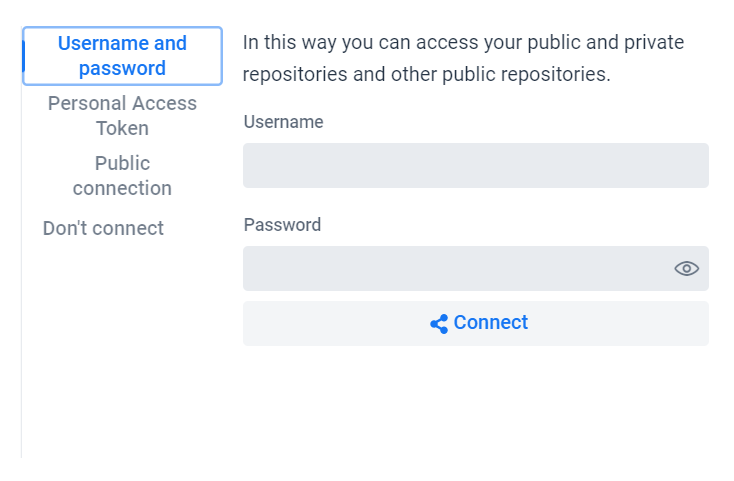
\includegraphics[width=\linewidth]{AnexE-MN-Fig1-1}
		\caption{Conexión mediante usuario y contraseña}
		\label{fig:dialogo-conexion_contraseña}
	\end{subfigure}\hfill
	\begin{subfigure}{.45\textwidth}
		\centering
		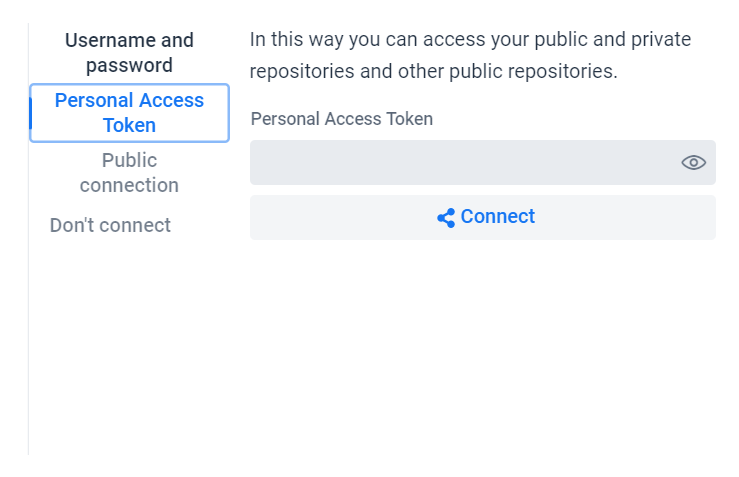
\includegraphics[width=\linewidth]{AnexE-MN-Fig1-2}
		\caption{Conexión mediante \textit{Personal Access Token}}
		\label{fig:dialogo-conexion_token}
	\end{subfigure}
	\begin{subfigure}{.45\textwidth}
		\centering
		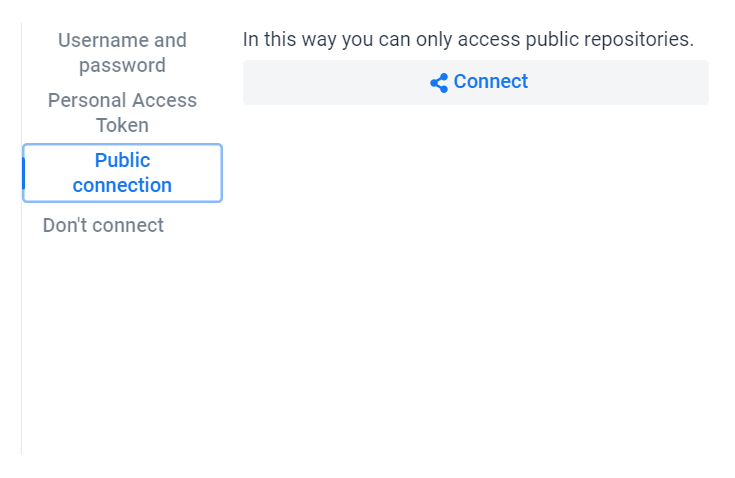
\includegraphics[width=\linewidth]{AnexE-MN-Fig1-3}
		\caption{Conexión publica}
		\label{fig:dialogo-conexion_publica}
	\end{subfigure}\hfill
	\begin{subfigure}{.45\textwidth}
		\centering
		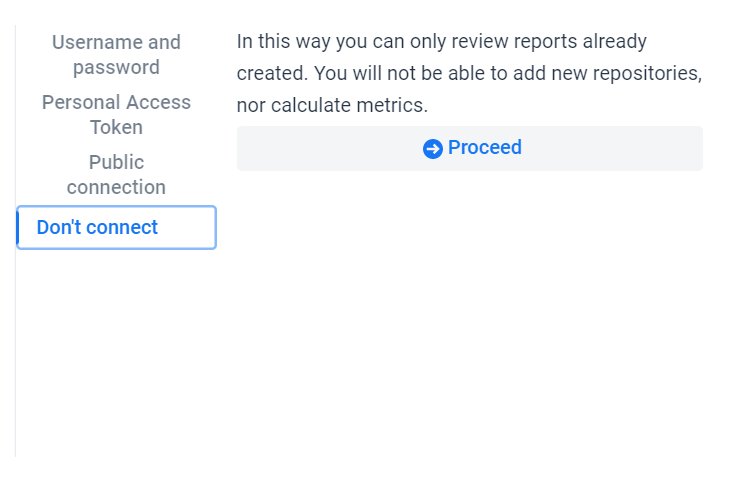
\includegraphics[width=\linewidth]{AnexE-MN-Fig1-4}
		\caption{Sin conexión}
		\label{fig:dialogo-conexion_sin-conexion}
	\end{subfigure}
	\caption{Distintas formas de establecer una conexión}
	\label{fig:AnexE-MN-Fig1-}
\end{figure}
Hay 4 posibilidades, que permiten establecer una conexión con la sesión iniciada (mediante usuario y contraseña o mediante \textit{PA Token}), una conexión pública o utilizar la aplicación sin conexión:
\begin{description}
	\tightlist
	\item[Iniciar sesión en GitLab mediante usuario y contraseña.] Se establece una conexión a GitLab iniciando sesión mediante un nombre de usuario y una contraseña. De esta forma se puede acceder a todos los repositorios públicos y privados accesibles por el usuario. Ver figura \ref{fig:dialogo-conexion_contraseña}.
	\item[Iniciar sesión en GitLab mediante \textit{Personal Access Token}.] Se establece una conexión a GitLab iniciando sesión mediante un \textit{Personal Access Token}. De esta forma se puede acceder a todos los repositorios públicos y privados accesibles por usuario, como ocurría en el caso anterior. 
	Si se accede a GitLab desde una \underline{cuenta externa} a GitLab como Google o GitHub, esta opción es la única manera de iniciar sesión con su cuenta de GitLab. Ver figura \ref{fig:dialogo-conexion_token}.\\
	Para generar un \textit{Personal Access Token} desde GitLab hay que iniciar sesión desde la web y entrar en la configuración del usuario. En el apartado de \textit{Access Token} se debe dar un nombre, opcionalmente una fecha de expiración y los permisos. Para utilizar la aplicación se necesitan estos permisos: \textit{api}, \textit{read\_user}, \textit{read\_repository}, \textit{read\_registry}. Una vez finalizado, pulsar sobre el botón "\textit{Create personal access token}", copiar el token y utilizarlo. Una vez se salga de la ventana en la que se muestra el token, no volverá a aparecer, por lo que se recomienda copiarlo en algún lado. Ver figura \ref{fig:AnexE-MN-Fig2}.
	\imagen{AnexE-MN-Fig2}{Crear un \textit{Personal Access Token} desde GitLab}
	\item[Usar una conexión pública hacia GitLab.] Se establece una conexión pública a GitLab sin iniciar sesión, por lo que solo se podrá acceder a repositorios públicos. Ver figura \ref{fig:dialogo-conexion_publica}.
	\item[No utilizar ninguna conexión.] No se realizará ninguna conexión a GitLab. Solo se podrá trabajar con proyectos y perfil de métricas importados y con el perfil de métricas por defecto. Ver figura \ref{fig:dialogo-conexion_sin-conexion}.
\end{description}

\subsection{Página principal}
\imagen{AnexE-MN-Fig3}{Página principal}
Una vez elegida por primera vez el tipo de conexión deseado se accede a la página principal, como se observa en la figura \ref{fig:AnexE-MN-Fig3}.
\subsubsection{Cambiar el tipo de conexión}
En la parte superior se puede observar el botón de conexión, que indica el tipo de conexión actual.
\begin{itemize}
	\tightlist
	\item Si se ha iniciado sesión mediante usuario y contraseña o mediante un \textit{personal access token}, se mostrará la imágen del usuario y el texto: ``Connected as: <nombre de usuario>''
	\item Si se ha establecido una conexión pública, se mostrara el texto: ``Using a public connection''
	\item Y si no se ha establecido ninguna conexión, el texto mostrado será: ``No connection to GitLab''.
\end{itemize}
Para cambiar el tipo de conexión es obligatorio cerrar, si existe, la conexión actual. Por ello, al pulsar sobre el botón de conexión, se muestra el diálogo de la figura \ref{fig:AnexE-MN-Fig4-1} si existe una conexión y el diálogo de la figura \ref{fig:AnexE-MN-Fig4-2} si no existe conexión. Al pulsar sobre ``\textit{Connect}'' o sobre ``\textit{Close connection}'' se abrirá el diálogo de conexión de las figuras \ref{fig:AnexE-MN-Fig1} y \ref{fig:AnexE-MN-Fig1-}.
\begin{figure}[!h]
	\centering
	\begin{subfigure}{.45\textwidth}
		\centering
		
\includegraphics[width=\linewidth]{AnexE-MN-Fig4-1}
		\caption{Cerrar conexión}
		\label{fig:AnexE-MN-Fig4-1}
	\end{subfigure}\hfill
	\begin{subfigure}{.45\textwidth}
		\centering
		
\includegraphics[width=\linewidth]{AnexE-MN-Fig4-2}
		\caption{Establecer conexión}
		\label{fig:AnexE-MN-Fig4-2}
	\end{subfigure}
	\caption{Modificar tipo de conexión}
	\label{fig:AnexE-MN-Fig4}
\end{figure}
\subsubsection{Botón de ayuda}
A la derecha del botón de conexión se encuentra un botón que da acceso a este manual en la Wiki del proyecto.
\subsubsection{Listado de proyectos}
En el centro de la página principal se pueden gestionar los proyectos. Consta de una barra de búsqueda, dos menús, y una tabla que visualiza las métricas de los proyectos que se añadan.

En el cuadro de búsqueda se filtrarán los repositorios por su nombre mientras se vaya escribiendo.

En el menú de ``\textit{Project management}'' existen estas opciones, como se muestra en la figura \ref{fig:AnexE-MN-Fig5-1}:
\begin{itemize}
	\item \textbf{\textit{Add new}.} Permite añadir uno o varios proyectos.
	\item \textbf{\textit{Import}.} Permite importar proyectos a partir de un fichero previamente exportado.
	\item \textbf{\textit{Export}.} Permite exportar todos los proyectos existentes a un fichero, lo que permitirá su posterior importación. Se almacena en un fichero con foromato ``.emr''.
	\item \textbf{\textit{Export to CSV}.} Permite generar un fichero CSV que contenga toda la información de la tabla de proyectos. Este fichero no servirá para importar los proyectos posteriormente.
\end{itemize}
En el menú de ``\textit{Evaluate projects}'' existen estas opciones, como se muestra en la figura \ref{fig:AnexE-MN-Fig5-2}:
\begin{itemize}
	\item \textbf{\textit{Evaluate with new profile}.} Permite evaluar los proyectos calculando los valores mínimos y máximos de cada métrica a partir de los repositorios actuales.
	\item \textbf{\textit{Evaluate with default profile}.} Permite evaluar los proyectos con un perfil por defecto creado a a partir de un conjunto de datos\footnote{\url{https://github.com/clopezno/clopezno.github.io/blob/master/agile_practices_experiment/DataSet_EvolutionSoftwareMetrics_FYP.csv}} de un estudio empírico de las métricas de evolución del software en trabajos finales de grado\cite{lopez_portal_2019}.
	\item \textbf{\textit{Evaluate with imported profile}.} Permite evaluar los proyectos a partir de un perfil de métricas previamente exportado.
	\item \textbf{\textit{Export actual profile}.} Permite exportar el perfil de métricas actual para su posterior importación. Se almacena en un fichero con foromato ``.emmp''.
\end{itemize}
\begin{figure}[!h]
	\centering
	\begin{subfigure}{.45\textwidth}
		\centering
		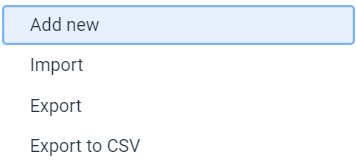
\includegraphics[width=\linewidth]{AnexE-MN-Fig5-1}
		\caption{Menú: ``\textit{Project management}''}
		\label{fig:AnexE-MN-Fig5-1}
	\end{subfigure}\hfill
	\begin{subfigure}{.45\textwidth}
		\centering
		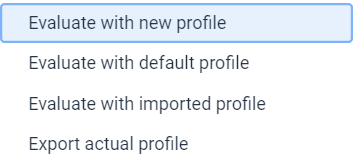
\includegraphics[width=\linewidth]{AnexE-MN-Fig5-2}
		\caption{Menú: ``\textit{Evaluate projects}''}
		\label{fig:AnexE-MN-Fig5-2}
	\end{subfigure}
	\caption{Menús del listado de repositorios}
	\label{fig:AnexE-MN-Fig5}
\end{figure}

La tabla muestra los valores medidos de las métricas para cada proyecto, ver figura \ref{fig:AnexE-MN-Fig8}.
\imagen{AnexE-MN-Fig8}{Tabla que muestra los valores medidos en los proyectos para las métricas}
La tabla presenta las siguientes columnas:
\begin{itemize}
	\item \textbf{Botón de eliminar.} Permite eliminar de la tabla el proyecto seleccionado.
	\item \textbf{\textit{Project}.} Nombre del proyecto con enlace al repositorio de GitLab. Si el nombre es demasiado largo y se corta, se puede utilizar el tooltip que aparece al pasar el ratón por encima del nombre del proyecto.
	\item \textbf{\textit{Date}.} Fecha de la última vez que se obtuvieron las métricas del proyecto.
	\item \textbf{Métricas.} Valor medido de las métricas y un color que evalúa la medida en relación a un perfil de métricas.\\
	Las métricas están clasificadas por categoría: Proceso de orientación (\textit{Process Orientation}) y Constantes de tiempo (\textit{Time Constraints}).\\
	En la cabecera se muestra el nombre de la métrica pero aparecerá la descripción al pasar el puntero del ratón por encima del nombre en forma de tooltip.
	Un \textbf{\underline{perfil de métricas}} es un conjunto de valores mínimo y máximo definidos para cada métrica. Los valores que se encuentran debajo del nombre de las métricas en la cabecera son esos valores mínimo y máximo separados por un guión para su respectiva métrica. En el tooltip se muestra el valor mínimo como Q1 y el valor máximo cómo Q3.
	
	\item \textbf{Botón de recalcular métricas.} Permite volver a obtener las métricas del proyecto (si es posible según la conexión actual a GitLab) y evaluar las nuevas métricas de acuerdo al perfil actual. Se mostrará un mensaje de aviso si se han recalculado correctamente y un mensaje de error en caso contrario.
\end{itemize}


\subsubsection{Añadir un proyecto}
Para añadir un nuevo proyecto, el tipo de conexión deberá ser distinto de ``Sin conexión'' (\textit{No connection to GitLab}), es decir que debe haber una conexión. Seleccionar la opción ``\textit{Add new}'' del menú ``\textit{Project management}'', ver figura \ref{fig:AnexE-MN-Fig5-1}. Se abrirá un diálogo como el de la figura \ref{fig:AnexE-MN-Fig6}. Para \underline{cancelar} se puede pulsar \textit{Esc} o hacer click fuera del diálogo.
\begin{figure}[!h]
	\centering
	\begin{subfigure}{.45\textwidth}
		\centering
		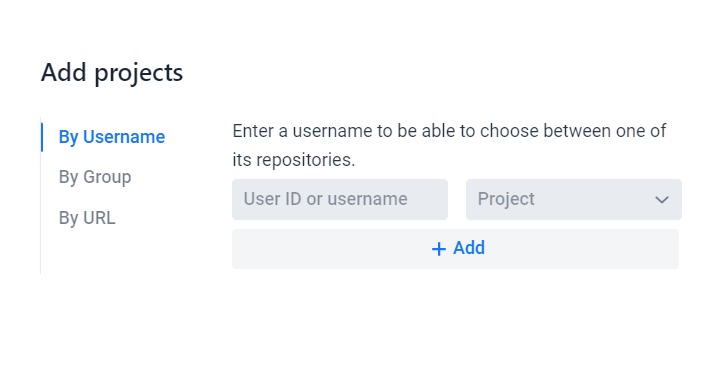
\includegraphics[width=\linewidth]{AnexE-MN-Fig6-1}
		\caption{Menú: ``\textit{Añadir por pertenencia a usuario}''}
		\label{fig:AnexE-MN-Fig6-1}
	\end{subfigure}\hfill
	\begin{subfigure}{.45\textwidth}
		\centering
		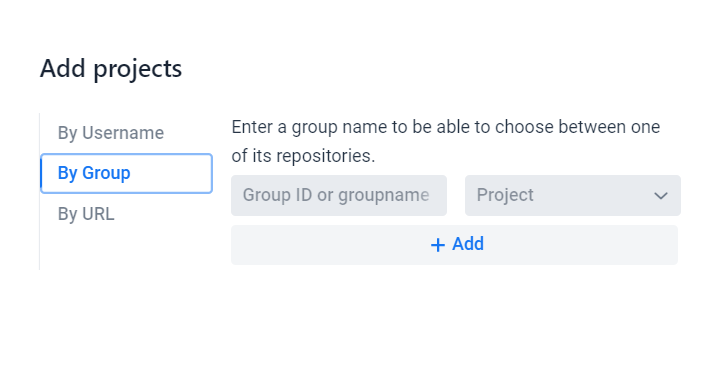
\includegraphics[width=\linewidth]{AnexE-MN-Fig6-2}
		\caption{Menú: ``\textit{Añadir por pertenencia a grupo}''}
		\label{fig:AnexE-MN-Fig6-2}
	\end{subfigure}
	\begin{subfigure}{.45\textwidth}
		\centering
		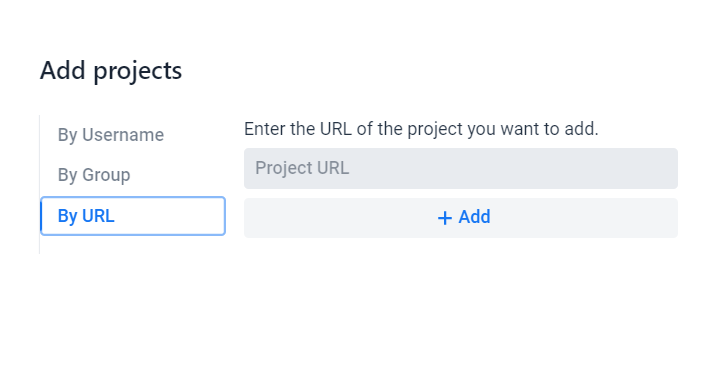
\includegraphics[width=\linewidth]{AnexE-MN-Fig6-3}
		\caption{Menú: ``\textit{Añadir proyecto por su URL Web}''}
		\label{fig:AnexE-MN-Fig6-3}
	\end{subfigure}
	\caption{Menús del listado de repositorios}
	\label{fig:AnexE-MN-Fig6}
\end{figure}
Existen tres posibilidades para añadir un proyecto:
\begin{description}
	\item[Añadir por pertenencia a un usuario.] Se solicita en el campo izquierdo del formulario el nombre de usuario o ID del usuario del cual se desean cargar los proyectos en campo desplegable de la derecha. Se mostrará un mensaje en rojo si el usuario no se existe ``\textit{User not found}'' y un mensaje si el usuario existe ``\textit{User found}'', en ese caso se cargarán todos los proyectos del usuario en el desplegable de la derecha. Seleccionar uno de sus proyectos y pulsar sobre el botón ``\textit{Add}''. Se mostrarán solo los repositorios públicos (incluyendo \textit{forks}) del usuario . No se mostrarán proyectos privados a menos que se haya establecido una conexión con sesión y el usuario especificado en el campo de la izquierda coincida con el usuario que haya iniciado sesión.
	\item[Añadir por pertenencia a un grupo.] El funcionamiento es el mismo que en el caso anterior, con la diferencia de que se solicita el nombre de grupo o ID del grupo en el campo izquierdo. Si el grupo es privado y el tipo de conexión es pública o el usuario que haya iniciado sesión no tiene acceso al grupo, se mostrará un mensaje en rojo de la misma forma que si el grupo no existiera ``\textit{Group not found}''. Si se encuentra el grupo, se mostrará el mensaje ``\textit{Group found}'' y se cargarán todos los proyectos del usuario en el desplegable de la derecha. Seleccionar uno de sus proyectos y pulsar sobre el botón ``\textit{Add}''.
	\item[Añadir por URL Web.] Se solicita la URL Web del proyecto de GitLab. Si no se encuentra (porque no existe o porque con la conexión actual no se tiene acceso al proyecto) se mostrará un mensaje en rojo al pulsar sobre ``\textbf{\textit{Add}}'': ``\textit{Project not found. It doesn't exists or may be inaccessible due to your connection level.}''
\end{description}
Al añadir un nuevo proyecto, se calcularán por primera vez sus métricas y se evaluarán de acuerdo al perfil de métricas actual. Si no se ha creado o importado ningún perfil, se evaluará según el perfil por defecto.
\subsubsection{Importar proyectos}
Los proyectos se pueden importar independientemente del tipo de conexión que exista. Se mostrará un diálogo que permite seleccionar o arrastrar al cuadro un fichero con formato \textit{.emr}, ver figura \ref{fig:AnexE-MN-Fig7}. Se puede seleccionar otro fichero en caso de haber escogido un fichero no deseado. Una vez se cargue el fichero, pulsar sobre ``Import''. Se mostrará un mensaje de error en caso de que el fichero este corrompido (ha sido modificado por una herramienta externa a la aplicación) y no se podrá utilizar ese fichero.
\begin{figure}[!h]
	\centering
	\begin{subfigure}{.45\textwidth}
		\centering
		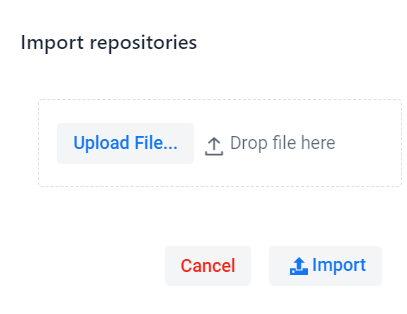
\includegraphics[width=\linewidth]{AnexE-MN-Fig7-1}
		\caption{Importar repositorios}
		\label{fig:AnexE-MN-Fig7-1}
	\end{subfigure}\hfill
	\begin{subfigure}{.45\textwidth}
		\centering
		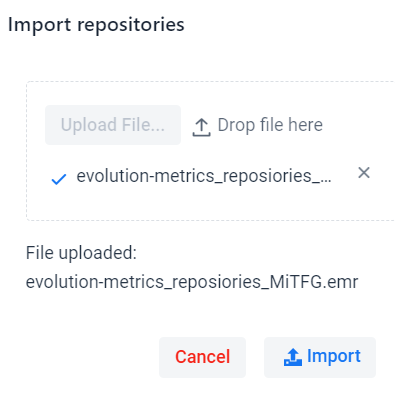
\includegraphics[width=\linewidth]{AnexE-MN-Fig7-2}
		\caption{Diálogo de importar con fichero cargado}
		\label{fig:AnexE-MN-Fig7-2}
	\end{subfigure}
	\caption{Diálogo para importar repositorios}
	\label{fig:AnexE-MN-Fig7}
\end{figure}
\subsubsection{Exportar proyectos}
Para exportar proyectos debe haber al menos un proyecto en la tabla.
Se puede exportar a un fichero \textit{.emr} para su posterior importación o en un fichero \textit{.csv}. Para exportar hay que seleccionar la opción correspondiente en el menú ``\textit{Project management}'', ver figura \ref{fig:AnexE-MN-Fig5-1}. El dialogo para la exportación se muestra en la figura \ref{fig:AnexE-MN-Fig9}. Basta con pulsar sobre ``\textit{Download}'' para poder descargar el fichero.
\begin{figure}[!h]
	\centering
	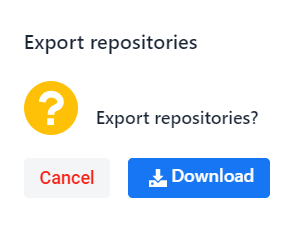
\includegraphics[scale=0.7]{AnexE-MN-Fig9}
	\caption{Diálogo de exportación}\label{fig:AnexE-MN-Fig9}
\end{figure}
\FloatBarrier
\subsubsection{Evaluar los proyectos}
Evaluar un proyecto es evaluar y todas las medidas de las métricas que se realizaron sobre el proyecto en relación a un perfil de métricas en el que se definen los valores mínimos y máximos.\\
El resultado de la evaluación puede ser bueno (la medida se pinta en verde en la tabla), malo (la medida se pinta en rojo) o ``advertencia'' (la medida equivale al valor mínimo o al valor máximo).

Para evaluar un proyecto hay que elegir el perfil de métricas con el que se va a evaluar. Por defecto se coge un perfil de métricas en el que los valores mínimos se corresponden con los quartiles Q1 y los valores máximos con cuartiles Q3 de un conjunto de medidas tomadas sobre TFGs\footnote{\url{https://github.com/clopezno/clopezno.github.io/blob/master/agile_practices_experiment/DataSet_EvolutionSoftwareMetrics_FYP.csv}}\cite{lopez_portal_2019}.

Al evaluar se evalúan todos los proyectos. Se puede elegir el perfil de métricas según la opción elegida en el menú ``\textit{Evaluate projects}'' de la figura \ref{fig:AnexE-MN-Fig5-2}:
\begin{itemize}
	\item \textbf{\textit{Evaluate with new profile}.} Coge como entrada todas las medidas de la tabla y calcula, por cada métrica, los cuartiles Q1 y Q3 para definirlos como valor mínimo y valor máximo de la métrica, respectivamente.
	\item \textbf{\textit{Evaluate with default profile}.} Permite evaluar los proyectos con el perfil por defecto mencionado anteriormente.
	\item \textbf{\textit{Evaluate with imported profile}.} Permite importar el perfil de métricas de un fichero \textit{.emmp}. El perfil se debe haber creado y exportado anteriormente.
\end{itemize}
\subsubsection{Exportar perfil de métricas}
Se puede exportar a un fichero \textit{.emmp} para su posterior importación. Para exportar el perfil de métricas, seleccionar la opción correspondiente del menú ``\textit{Evaluate projects}'' de la figura \ref{fig:AnexE-MN-Fig5-2}: ``\textit{Export actual profile}''. El diálogo para la exportación es similar al de la figura \ref{fig:AnexE-MN-Fig9}. Basta con pulsar sobre ``\textit{Download}'' para poder descargar el fichero que contendrá el perfil de métricas actual.